\documentclass{article}
\usepackage[utf8]{inputenc}
\usepackage{amsmath,amssymb}
\usepackage{amsfonts}
\usepackage{paralist}
\usepackage{color}
\usepackage[table]{xcolor}
\usepackage{graphicx}
\usepackage[detect-weight=true, binary-units=true]{siunitx}
\usepackage{pgfplots}
\usepackage{authblk}
\usepackage{float}
\usepackage{url}
\usepackage{multirow}
\usepackage{booktabs}
\usepackage{blindtext}
\usepackage{hyperref}

\usepackage{geometry}
\geometry{margin = 1.5 in}

\usepackage{listings}
\usepackage{xcolor}
\definecolor{codekeyword}{rgb}{0.0, 0.5, 0.0} % Dark green
\definecolor{codestring}{rgb}{0.58, 0.0, 0.82} % Purple
\definecolor{codecomment}{rgb}{0.5, 0.5, 0.5} % Gray
\definecolor{background}{rgb}{0.95, 0.95, 0.95} % Light gray
\lstnewenvironment{sql}[1][]{
    \lstset{
        language=SQL,
        basicstyle=\small\ttfamily,
        numbers=none,
        numberstyle=\tiny\color{gray},
        keywordstyle=\color{codekeyword},
        stringstyle=\color{codestring},
        commentstyle=\color{codecomment},
        morekeywords={
            SELECT, FROM, WHERE, GROUP BY, ORDER BY, EXTRACT, INSERT, 
            UPDATE, DELETE, CREATE, ALTER, DROP, JOIN, INNER, LEFT, RIGHT, 
            FULL, ON, DISTINCT, INTO, VALUES, SET, AS, AND, OR, NOT, IN, 
            LIKE, IS, NULL, UNION, ALL, HAVING, BETWEEN, EXISTS, OVER, PARTITION},
        breaklines=true,
        frame=single,
        framesep=3pt,
        frameround=tttt,
        backgroundcolor=\color{gray!10},
        rulecolor=\color{black!30},
        tabsize=4,
        columns=flexible,
        %captionpos=b,
        title=#1,
        literate={\ }{{\space}}1
    }
}{}


\title{Data Management - Final Project}
\author{Sara Carpenè, Alessio Valentinis, Marco Zampar}
%\date{July 2024}

\begin{document}

\maketitle

%Introduction
\section{Introduction}

This project has the aim of optimize a set of four queries from the \href{www.tpc.org/tpc\_documents\_current\_versions/pdf/tpch\_v3.0.1.pdf}{TPC benchmark H}
The database consists of eight tables: customer, lineitem,
nation, orders, part, partsupp, region, supplier. The relations between tables can be seen in the schema in figure \ref{fig:rel_schema}.

\begin{figure}[h!]
    \centering
    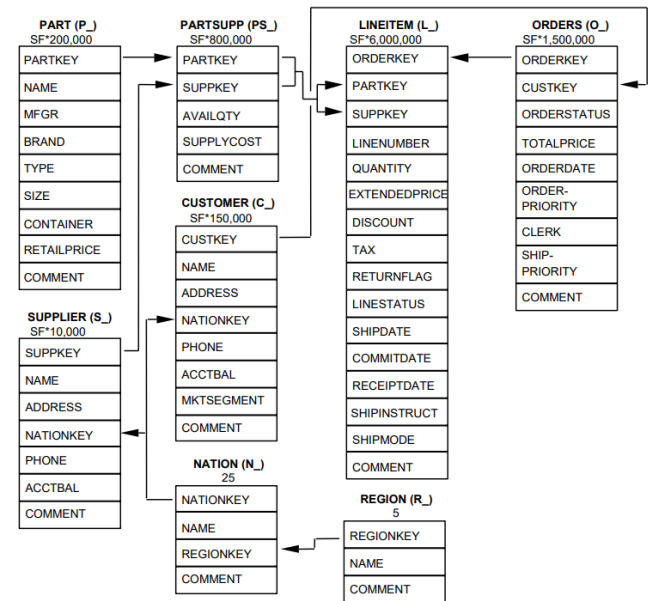
\includegraphics[scale=0.45]{images/rel_schema.png}
    \caption{Schema of the relaction between tables in the TPC-H benchmark}
    \label{fig:rel_schema}
\end{figure}

\subsection{Creation and population of the database}

The size of the database is scalable, and depends on a scale factor (SF), and we were given data generated from $SF=10$. Each table, from the documentation, has its own primary key and one or more foreign keys. Complete description of the table can be found \href{www.tpc.org/tpc\_documents\_current\_versions/pdf/tpch\_v3.0.1.pdf}{here}, while the complete SQL tables implementation and creation can be found \href{https://github.com/ValentinisAlessio/DM_Final_Project/blob/main/dbms.ipynb}{here}.

For the purpose of space economy, we opted for an initial "vanilla" creation of the tables, without any kind of keys: this choice is furthermore supported by the fact that we are dealing with a Data Warehousing context, so we expect the data to be already prepared and cleaned from duplicates.

After having populated the tables, we inserted all the keys reported in the documentation in order to work properly with the relations. However, always for the purpose of gaining some space, we decided not to implement the \textit{Primary key} to the Main table \texttt{lineitem}, as (for the same purposes described above,) we don't need to check for uniqueness constraints during the population of the Database, and for the sake of optimization, a simple index should help us to spare some pretty useful space.

In the table \ref{tab:table_dimensions}, we provide some information about the dimension of the various tables, in increasing order.

\begin{table}[h!]
\centering
\begin{tabular}{c|c|c|c}
\rowcolor{blue!50} Table & Number of rows & Dim without keys (MB) & Dim with keys (MB)\\
\rowcolor{gray!10} region & 5 & 0.01 & 0.02\\ 
\rowcolor{white} nation & 25 & 0.01 & 0.02\\ 
\rowcolor{gray!10} supplier & 100000 & 17.35  & 19.51 \\ 
\rowcolor{white} customer & 1500000& 290.17  & 322.32 \\ 
\rowcolor{gray!10} part & 2000000 & 320.14  & 363.00 \\ 
\rowcolor{white} partsupp & 8000000 & 1362.80  & 1535.12 \\
\rowcolor{gray!10} orders & 15000000 & 2038.97  & 2360.30 \\
\rowcolor{white} lineitem & 59986052 & 8787.95  & 10073.67 \\
\end{tabular}\\[0.5cm]
    \caption{General statistics}
    \label{tab:table_dimensions}
\end{table}

%Statistics
\section{Statistics of the DB}
In this section, we will present some useful statistics of the database.

The original database has a total dimension of 14681.63 MB (?? $13.075 GB$ ??), this encompasses both the physical size of the tables and the dimensions of primary and secondary indexes across various attributes.

%SISTEMERO' IL RIFERIMENTO
In section \ref{appdx:stats} it can be found the complete statistics of the tables detailing its attributes along with the count of unique values, minimum, and maximum values for each attribute.

Here, to keep the focus on the four queries that we want to optimize, we will limit the presentation to some of that statistics. Specifically we decided to mention only the tables and the attributes that will be involved in at least one of the chosen query. 


\begin{table}[H]
\centering
\begin{tabular}{c|c|c|c}
\rowcolor{blue!50} Attribute & Distinct values & Min value & Max value\\
\rowcolor{gray!10} \textbf{c\_custkey} & 1500000 & 1 & 1500000 \\ 
\rowcolor{white} c\_name & 1500000 & 'Customer\#000000001' & 'Customer\#001500000'\\ 
\rowcolor{gray!10} c\_address & 1500000 & - & - \\ 
\rowcolor{white} c\_nationkey & 25 & 0 & 24\\ 
\rowcolor{gray!10} c\_phone & 1499963 & - & - \\
\rowcolor{white} c\_acctbal & 818834 & '-999.99' & '9999.99' \\
%\rowcolor{gray!10} c\_mktsegment & 5 & - & - \\
\rowcolor{gray!10} c\_comment & 1496636 & - & - \\
\end{tabular}\\[0.5cm]
    \caption{Costumer statistics}
    \label{tab:costumer_stats}
\end{table}


\begin{table}[H]
\centering
\begin{tabular}{c|c|c|c}
\rowcolor{blue!50} Attribute & Distinct values & Min value & Max value\\
\rowcolor{gray!10} \textbf{p\_partkey} & 2000000 & 1 & 2000000 \\
\rowcolor{white} p\_type & 150 & - & - \\
\rowcolor{gray!10} p\_container & 40 & - & - \\
\end{tabular}\\[0.5cm]
    \caption{Part statistics}
    \label{tab:part_stats}
\end{table}


\begin{table}[H]
\centering
\begin{tabular}{c|c|c|c} 
\rowcolor{blue!50} Attribute & Distinct values & Min value & Max value \\
\rowcolor{gray!10} \textbf{l\_orderkey} & 15000000 & 1 & 60000000 \\ 
\rowcolor{white} l\_partkey & 2000000 & 1 & 2000000 \\
\rowcolor{gray!10} l\_quantity & 50 & 1 & 50 \\
\rowcolor{white} l\_extendedprice & 1351462 & 900.91 & 104949.5 \\
\rowcolor{gray!10} l\_discount & 11 & '0.0' & '0.1' \\
\rowcolor{white} l\_tax & 9 & '0.0' & '0.08' \\
\rowcolor{gray!10} l\_returnflag & 3 & - & - \\
\rowcolor{white} l\_linestatus & 2 & - & - \\
\rowcolor{gray!10} l\_shipdate & 2526 & '1992-01-02' & '1998-12-01' \\
\rowcolor{white} \textbf{l\_linenumber} & 7 & 1 & 7 \\
\end{tabular}\\[0.5cm]
    \caption{Lineitem statistics}
    \label{tab:lineitem_stats}
\end{table}

\begin{table}[H]
\centering
\begin{tabular}{c|c|c|c} 
\rowcolor{blue!50} Attribute & Distinct values & Min value & Max value \\
\rowcolor{gray!10} \textbf{o\_orderkey} & 15000000 & 1 & 60000000 \\
\rowcolor{white} o\_custkey & 999982 & 1 & 1499999 \\
%\rowcolor{gray!10} o\_orderstatus & 3 & - & - \\
%\rowcolor{white} o\_totalprice & 11944103 & '838.05' & '558822.56' \\
\rowcolor{gray!10} o\_orderdate & 2406 & '1992-01-01' & '1998-08-02' \\
%\rowcolor{white} o\_orderpriority & 5 & - & - \\
\end{tabular}\\[0.5cm] 
    \caption{Orders statistics}
    \label{tab:orders_stats}
\end{table}



\begin{table}[H]
\centering
\begin{tabular}{c|c|c|c} 
\rowcolor{blue!50} Attribute & Distinct values & Min value & Max value \\
\rowcolor{gray!10} \textbf{n\_nationkey} & 25 & 0 & 24 \\
\rowcolor{white} n\_name & 25 & - & - \\
\end{tabular}\\[0.5cm]
    \caption{Nation statistics}
    \label{tab:nation_stats}
\end{table}

%% FORSE DI QUESTE TABELLE SAREBBE BENE, PER MAGGIORE CHIAREZZA, TENERE SOLO GLI ATTRIBUTI CHE SONO FK O CHE SONO USATI NELLE QUERY, SENNò VIENE TUTTO UN CASOTTO

%Queries

\section{Query schemas}

The assignment consists in using TPC-Benchmark H to test and optimize a set of four queries, using indexes, materialized views, a mixed approach of the two and fragmentation.

The set of queries selected for the assignment are Q1, Q10, Q14, Q17 of the Official Documentation. An overall view on the description and SQL implementation is given below.

\subsection{Query 1}
\textbf{Brief description}
The Pricing Summary Report Query provides a summary pricing report for all lineitems shipped as of a given date.
The date is within 60 - 120 days of the greatest ship date contained in the database. The query lists totals for
extended price, discounted extended price, discounted extended price plus tax, average quantity, average extended
price, and average discount. These aggregates are grouped by RETURNFLAG and LINESTATUS, and listed in
ascending order of RETURNFLAG and LINESTATUS. A count of the number of lineitems in each group is
included.

\textbf{Functional definition}
\begin{sql}
SELECT
    l_returnflag,
    l_linestatus,
    SUM(l_quantity) AS sum_qty,
    SUM(l_extendedprice) AS sum_base_price,
    SUM(l_extendedprice * (1 - l_discount)) AS sum_disc_price,
    SUM(l_extendedprice * (1 - l_discount) * (1 + l_tax)) AS sum_charge,
    AVG(l_quantity) AS avg_qty,
    AVG(l_extendedprice) AS avg_price,
    AVG(l_discount) AS avg_disc,
    COUNT(*) AS count_order
FROM
    lineitem
WHERE
    l_shipdate <= DATE '1998-12-01' - INTERVAL '[DELTA]' DAY
GROUP BY
    l_returnflag,
    l_linestatus
ORDER BY
    l_returnflag,
    l_linestatus;
\end{sql}

For a matter of simplicity we decided to take as slicing values the ones proposed by the validation paragraph in the official documentation. (So

\verb|'[DELTA]' = '90'|)

\subsection{Query 10}
\textbf{Brief description}
The Returned Item Reporting Query finds the top 20 customers, in terms of their effect on lost revenue for a given
quarter, who have returned parts. The query considers only parts that were ordered in the specified quarter. The
query lists the customer's name, address, nation, phone number, account balance, comment information and revenue
lost. The customers are listed in descending order of lost revenue. Revenue lost is defined as
sum(l\_extendedprice*(1-l\_discount)) for all qualifying lineitems.

\textbf{Functional definition}
\begin{sql}
SELECT
    c_custkey,
    c_name,
    SUM(l_extendedprice * (1 - l_discount)) AS revenue,
    c_acctbal,
    n_name,
    c_address,
    c_phone,
    c_comment
FROM
    customer,
    orders,
    lineitem,
    nation
WHERE
    c_custkey = o_custkey
    AND l_orderkey = o_orderkey
    AND o_orderdate >= DATE '[DATE]'
    AND o_orderdate < DATE '[DATE]' + INTERVAL '3' MONTH
    AND l_returnflag = 'R'
    AND c_nationkey = n_nationkey
GROUP BY
    c_custkey,
    c_name,
    c_acctbal,
    c_phone,
    n_name,
    c_address,
    c_comment
ORDER BY
    revenue DESC;
\end{sql}

For a matter of simplicity we decided to take as slicing values the ones proposed by the validation paragraph in the official documentation. (So

\verb|'[DATE]' = '1993-10-01'|)

\subsection{Query 14}
\textbf{Brief description}
The Promotion Effect Query determines what percentage of the revenue in a given year and month was derived from 
promotional parts. The query considers only parts actually shipped in that month and gives the percentage. Revenue 
is defined as (l\_extendedprice * (1-l\_discount)).


\textbf{Functional definition}
\begin{sql}
SELECT 
    100.00 * SUM (CASE WHEN p_type like 'PROMO%' 
                  THEN l_extendedprice*(1-l_discount) 
                  ELSE 0 END) / SUM(l_extendedprice * (1 - l_discount)) 
    AS promo_revenue
FROM 
    lineitem, 
    part
WHERE 
    l_partkey = p_partkey
    AND l_shipdate >= date '[DATE]'
    AND l_shipdate < date '[DATE]' + interval '1' month;

\end{sql}

For a matter of simplicity we decided to take as slicing values the ones proposed by the validation paragraph in the official documentation. (So \verb|'[DATE]' = '1995-09-01'|)


\subsection{Query 17}

\textbf{Brief description}
The Small-Quantity-Order Revenue Query considers parts of a given brand and with a given container type and 
determines the average lineitem quantity of such parts ordered for all orders (past and pending) in the 7-year database. What would be the average yearly gross (undiscounted) loss in revenue if orders for these parts with a quantity 
of less than 20 \% of this average were no longer taken?

\textbf{Functional definition}
\begin{sql}
SELECT
    SUM(l_extendedprice) / 7.0 AS avg_yearly
FROM 
    lineitem, 
    part
WHERE 
    p_partkey = l_partkey
    AND p_brand = '[BRAND]'
    AND p_container = '[CONTAINER]'
    AND l_quantity < ( 
                        SELECT 
                            0.2 * AVG(l_quantity)
                        FROM 
                            lineitem
                        WHERE 
                            l_partkey = p_partkey
                      );

\end{sql}

For a matter of simplicity we decided to take as slicing values the ones proposed by the validation paragraph in the official documentation. (So 

\verb|'[BRAND]' = 'Brand#23'| and \verb|'[CONTAINER]' = 'MED BOX'|)

%Baseline
\section{Baseline}

We decided to test the execution time of queries without additional indexes or views, other than the keys suggested by the documentation, and to use it as a baseline for further improvement in the management of the queries.

We obtained the execution times using the \emph{EXPLAIN ANALYZE} function available in PostgreSQL. The times represent the total estimated cost to execute the (entire) query. They are the sum of the startup cost and the cost to process all rows.

Every query has been tested five times, in order to record the mean and the standard deviation of the execution time, leading to more robust results.

The results of the tests are reported in the plot at table \ref{tab:baseline_exec_time}.
[ADD COMMENT ON THE QUERY 17 RESULTS]

\begin{table}[H]
\centering 
\begin{tabular}{c|c|c} 
\rowcolor{blue!50} Query & Mean & Std\\ 
\rowcolor{gray!10} Q. 1 &41.778 &1.412\\
\rowcolor{white} Q. 10 &33.077 &1.634\\
\rowcolor{gray!10} Q. 14 &28.253 &1.239\\
\rowcolor{white} Q. 17 &N/A &N/A \\
\end{tabular}\\[0.5cm] 
\caption{Execution times of query} 
\label{tab:baseline_exec_time} 
\end{table}



%Indexes
\section{Indexes}

Our first attempt was to add indexes on foreign keys, but in almost all cases, they weren't used, or didn't bring too many advantages, compared with their size.

For the sake of completeness we will report anyway the results (???).

Our second attempt was to add indexes on the attributes used for slicing, so involved in the \verb|WHERE| condition.

\begin{table}[H]
\centering
\begin{tabular}{c|c|c|c|c}
\rowcolor{blue!50} Table & Attribute & Used in Query & Creation time [s] & Index size [MB]\\
\rowcolor{gray!10} lineitem & l\_shipdate & Q1 & 32.43 & 397.54\\ 
\rowcolor{white} lineitem & l\_returnflag & Q1 & 61.83 & 396.46\\ 
\rowcolor{gray!10} lineitem & l\_partkey & Q17 & 46.99 & 429.50\\ 
\rowcolor{white} orders & o\_orderdate & Q10 & 8.10 & \\ 
\end{tabular}\\[0.5cm]
    \caption{Indexes dimensions}
   % \label{tab:costumer_stats}
\end{table}

With these indexes, which are ensured to be used in the execution of the queries, resulted in a total database size of $20.55 GB$.

The execution time of the queries is summarized in the table below.

\begin{table}[H]
\centering
\begin{tabular}{c|c|c}
\rowcolor{blue!50} Query & Mean & Std\\
\rowcolor{gray!10} Q1     &30.009                &1.224\\
\rowcolor{white} Q10    &25.677               &1.799\\
\rowcolor{gray!10} Q14    &23.607               &0.327\\
\rowcolor{white} Q17    &11.232               &0.967 \\
\end{tabular}\\[0.5cm]
    \caption{Execution times of query with indexes}
    \label{tab:idx_exec_time}
\end{table}


%Materialized view
\section{Materialized views}
In this section we will propose some materialized views that aim to improve the execution time of the chosen queries. For the creation of this views we enabled all the hash related operations, since the main purpose of the section is to evaluate performances related to  materialization of some tables, rather than delving into the specifics of this process.

\subsection{Lineitem-part}
\label{ssec:lineitem-part}
In order to improve performances in executing query 14 we decided to create a materialized view as follow:
\begin{sql}
CREATE MATERIALIZED VIEW part_lineitem AS
SELECT
    l_returnflag,
    l_linestatus,
    l_quantity,
    l_extendedprice,
    l_discount,
    l_tax,
    l_shipdate,
    l_partkey,
    p_partkey,
    p_brand,
    p_container,
    SUBSTRING(p_type FROM 1 FOR 5) AS p_type_prefix,
    0.2 * AVG(l_quantity) OVER (PARTITION BY l_partkey) AS avg_quantity
FROM
    lineitem l
JOIN
    part p ON l.l_partkey = p.p_partkey;
\end{sql}

\textbf{Statistics of this view:}
\begin{itemize}
    \item Required time to create the view 310.952 seconds.
    \item Size of the view: 6.43 GB.
\end{itemize}

We rewrote the query 14 and 17 in order to exploit the materialized views.


Materializing the join operation of query 14 we expected to have a lower execution time with respect to the baseline, but this did not happened. By observing the output of the \emph{EXPLAIN ANALYZE} function we understood that the problem with the lack of gain in performance is that the optimizer performs a sequential scan of the lineitem table, since there is no index on shipdate.

The greatest improvement in using this materialization was expected to be in query 17. Indeed the execution time dropped to 15.265 seconds (on a single run), which is a sensible gain in terms of performances. 

\subsection{Costumer-orders-lineitem-nation}
\label{ssec:costumer-orders-lineitem-nation}
In order to spare the most time of the joins in query 10 we created a bigger materialized view.
\begin{sql}
CREATE MATERIALIZED VIEW customer_order_lineitem_nation AS
SELECT
    c.c_custkey,
    c.c_name,
    c.c_acctbal,
    n.n_name,
    c.c_address,
    c.c_phone,
    c.c_comment,
    l.l_returnflag,
    l.l_discount,
    l.l_extendedprice,
    o.o_orderdate

FROM
    customer c
JOIN
    orders o ON c.c_custkey = o.o_custkey
JOIN
    lineitem l ON l.l_orderkey = o.o_orderkey
JOIN
    nation n ON c.c_nationkey = n.n_nationkey;
\end{sql}

\textbf{Statistics of this view:}
\begin{itemize}
    \item Required time to create the view 437.107 seconds.
    \item Size of the view: 12.63 GB.
\end{itemize}


We tested the performances of query 10 rewritten using this materialization, but there was no gain in efficiency, other than the fact that this materialization was made ad-hoc for this single query.

\subsection{Lineitem-part-orders}
As a last option we opted for a mixed approach creating a view which is neither as big nor as specific as the previous ones.

\begin{sql}
CREATE MATERIALIZED VIEW part_lineitem_order AS
SELECT
    l_returnflag,
    l_linestatus,
    l_quantity,
    l_extendedprice,
    l_discount,
    l_tax,
    l_shipdate,
    l_partkey,
    p_partkey,
    p_brand,
    p_container,
    SUBSTRING(p_type FROM 1 FOR 5) AS p_type_prefix,
    0.2 * AVG(l_quantity) OVER (PARTITION BY l_partkey) AS avg_quantity,
    o_orderkey,
    o.o_custkey,
    o.o_orderdate
FROM
    lineitem l
JOIN
    part p ON l.l_partkey = p.p_partkey
JOIN
    orders o ON l.l_orderkey = o.o_orderkey;
\end{sql}

\textbf{Statistics of this view:}
\begin{itemize}
    \item Required time to create the view 366.508 seconds.
    \item Size of the view: 6.93 GB.
\end{itemize}

As this is the expected best materialization, we report the modified queries that use it.

\begin{sql}[Query 10]
SELECT
    c_custkey,
    c_name,
    SUM(l_extendedprice * (1 - l_discount)) AS revenue,
    c_acctbal,
    n_name,
    c_address,
    c_phone,
    c_comment
FROM
    part_lineitem_order
    JOIN customer c ON c.c_custkey = o_custkey
    JOIN nation n ON c.c_nationkey = n.n_nationkey
WHERE
    o_orderdate >= DATE '1993-10-01'
    AND o_orderdate < DATE '1993-10-01' + INTERVAL '3' MONTH
    AND l_returnflag = 'R'
GROUP BY
    c_custkey,
    c_name,
    c_acctbal,
    c_phone,
    n_name,
    c_address,
    c_comment
ORDER BY
    revenue DESC;
\end{sql}

\begin{sql}[Query 14]
SELECT
    100.00 * SUM(CASE
        WHEN p_type_prefix LIKE 'PROMO'
        THEN l_extendedprice * (1 - l_discount)
        ELSE 0
    END) / SUM(l_extendedprice * (1 - l_discount)) AS promo_revenue
FROM
    part_lineitem_order
WHERE
    l_shipdate >= DATE '1995-09-01'
    AND l_shipdate < DATE '1995-09-01' + INTERVAL '1' MONTH;
\end{sql}

\begin{sql}[Query 17]
SELECT
    SUM(l_extendedprice) / 7.0 AS avg_yearly
FROM
    part_lineitem_order
WHERE
    p_brand = 'Brand#23'
    AND p_container = 'MED BOX'
    AND l_quantity < avg_quantity;
\end{sql}

In this case we performed a complete benchmark, and the results are reported in the table below \ref{tab:materialize}.

\begin{table}[H]
\centering 
\begin{tabular}{c|c|c} 
\rowcolor{blue!50} Query & Mean & Std\\
\rowcolor{gray!10} Q1 &24.770 &2.034\\
\rowcolor{white} Q10 &50.135 &59.566\\
\rowcolor{gray!10} Q14 &20.677 &0.353\\
\rowcolor{white} Q17 &20.465 &0.655\\
\end{tabular}\\[0.5cm] 
\caption{Execution times of query with materialized views} 
\label{tab:materialize} 
\end{table}

For the sake of completeness, we will briefly present an idea to optimize with materialization also query one, which is the only query in the chosen set that isn't directly influenced by the already introduced materialized views.
We proposed a materialization that returns a "slimmer" version of the lineitem table with less attributes than the original one. Specifically we decided to keep only l\_returnflag, l\_linestatus, l\_extendedprice,l\_discount, l\_tax, l\_quantity. 

This approach leaded to a slight decrease in the execution time of query 1, but this improvement was not so significant to balance the size of the materialized view and its specificity. Indeed this materialization is "taylored" to query 1 and it could hardly be used in the optimization of other queries.

Since, in completing this project, we have always considered our set of four queries as a small subset of the possible query that a company may see as interesting in the decision making process, we didn't want to burden the database with too specific materialized views. For this reason we decided to not consider also this materialization, and to continue the project with only the materialized view that involves lineitem, part and orders tables.




%Index e materialized
\section{Mixed approach}
In this section we explored a mixed approach with both materialization and indexing.
As we already sapred the join conditions, we will just consider indexes that are useful for slicing.
Remember that the chosen materialized view results to be \textit{Lineitem-part-orders}, but for the sake of completeness, we reported also indexing on all the materialization attempts, in order to record possible time improvement. 

For every materialization we will report a table with the introduced indexes and their creation time and size.

\subsection{Lineitem-part}

\begin{table}[H]
\centering
\begin{tabular}{c|c|c}
\rowcolor{blue!50}  Attribute     & Creation time [s] & Index size [MB]\\
\rowcolor{gray!10} l\_shipdate     & 30.16          & 397.55 \\ 
\rowcolor{white}   p\_brand        & 58.95          & 403.14 \\
\rowcolor{gray!10} p\_container    & 60.34          & 403.15 \\ 
\end{tabular}\\[0.5cm]
    \caption{Indexes dimensions}
   % \label{tab:costumer_stats}
\end{table}
Using this indexes the total size of tables is: 7.60 GB.

Remember that this materialization is useful mainly for queries 14 and 17, so the indexes were placed on the suitable slicing attributes.

\subsection{Costumer-orders-lineitem-nation}

\begin{table}[H]
\centering
\begin{tabular}{c|c|c}
\rowcolor{blue!50}  Attribute     & Creation time [s] & Index size [MB]\\
\rowcolor{gray!10} o\_orderdate     & 58.30       & 397.51 \\ 
\rowcolor{white}   l\_returnflag    & 50.62       & 396.46 \\
\end{tabular}\\[0.5cm]
    \caption{Indexes dimensions}
   % \label{tab:costumer_stats}
\end{table}
Using this indexes the total size of tables is: 13.41 GB.

Recalling that this materialization is pretty useful only for one query, we exploited indexing only for the proper attributes, but given the resulting size of the table, we furthermore opted for dropping this big materialization in favor of smaller ones.

\subsection{Lineitem-part-orders}

\begin{table}[H]
\centering
\begin{tabular}{c|c|c}
\rowcolor{blue!50}  Attribute       & Creation time [s] & Index size [MB]\\
\rowcolor{gray!10} l\_shipdate      & 47.12          & 397.55 \\ 
\rowcolor{white} o\_orderdate       & 44.72          & 397.51 \\ 
\rowcolor{gray!10} l\_returnflag    & 47.30          & 396.46 \\
\rowcolor{white}   p\_brand         & 49.68          & 403.14 \\
\rowcolor{gray!10} p\_container     & 59.57          & 403.15 \\ 
\end{tabular}\\[0.5cm]
    \caption{Indexes dimensions}
   % \label{tab:costumer_stats}
\end{table}

Using this indexes the total size of tables is: 8.11 GB.

As this materialization resulted to be useful for three of the four proposed queries, we added indexes for all the useful slicing attributes involved in queries 10, 14, 17.

Recalling the fact that the chosen final materialization is the \textit{lineitem-part-orders}, with all the indexes the final database size is of 32.23 GB.

We reported in table \ref{tab_mixed} the results of testing the queries with the described structure.



\begin{table}[H] 
\centering \begin{tabular}{c|c|c} 
\rowcolor{blue!50} Query & Mean & Std\\
\rowcolor{gray!10} Q1 &23.184 &1.360\\
\rowcolor{white} Q10 &34.227 &4.548\\
\rowcolor{gray!10} Q14 &24.086 &1.504\\
\rowcolor{white} Q17 &1.587 &0.103\\
\end{tabular}\\[0.5cm] 
\caption{Execution times of query with both materialized views and indexes} 
\label{tab:mixed} 
\end{table}

%Fragmentation
\section{Fragmentation}
We considered to implement the fragmentation only for the tables of lineitem and orders since they are the most computationally expansive to scan entirely and since they are strictly involved in the set of our chosen queries.

While designing the fragmentation, we have always considered the broader aspect of the database as a decision-making tool, avoiding introducing too specific partitions that could have improved the specific set of chosen queries, but would have unnecessarily burdened the database as they were not generalizable to other queries. Therefore, we decided to consider a temporal fragmentation, as the temporal dimension is often involved in slicing conditions, even outside of the chosen queries. 

In particular we fragmented the orders table with respect to the \textbf{o\_orderdate} attribute. Each partitioned table contains a time-span of three months to allow a significant improvement in executing query 10. Furthermore we introduced in the partitioned tables a primary key in o\_orderkey and a foreign key on o\_custkey referencing c\_custkey.

For the lineitem table we decided to use a partition on \textbf{l\_shipdate} and a sub-partition on \textbf{l\_returnflag}, to allow exploiting this partitioning in query 1, 10, 14.

The results are reported in the table \ref{tab:fragm_exec_time}

\begin{table}[H]
\centering 
\begin{tabular}{c|c|c} 
\rowcolor{blue!50} Query & Mean & Std\\
\rowcolor{gray!10} Q1 &60.109 &4.050\\
\rowcolor{white} Q10 &19.369 &4.091\\
\rowcolor{gray!10} Q14 &3.834 &0.160\\
\rowcolor{white} Q17 &311.702 &85.586\\
\end{tabular}\\[0.5cm] 
\caption{Execution times of query with fragmented db} 
\label{tab:fragm_exec_time} 
\end{table}


%Conclusions
\section{Conclusions}

\newpage
% Appendix
\appendix
\section{Appendix A}
\label{appdx:stats}
Complete statistics of the database.

\begin{table}[H]
\centering
\begin{tabular}{c|c|c|c}
\rowcolor{blue!50} Attribute & Distinct values & Min value & Max value\\
\rowcolor{gray!10} \textbf{c\_custkey} & 1500000 & 1 & 1500000 \\ 
\rowcolor{white} c\_name & 1500000 & 'Customer\#000000001' & 'Customer\#001500000'\\ 
\rowcolor{gray!10} c\_address & 1500000 & - & - \\ 
\rowcolor{white} c\_nationkey & 25 & 0 & 24\\ 
\rowcolor{gray!10} c\_phone & 1499963 & - & - \\
\rowcolor{white} c\_acctbal & 818834 & '-999.99' & '9999.99' \\
\rowcolor{gray!10} c\_mktsegment & 5 & - & - \\
\rowcolor{white} c\_comment & 1496636 & - & - \\
\end{tabular}\\[0.5cm]
    \caption{Costumer statistics}
   % \label{tab:costumer_stats}
\end{table}

\begin{table}[H]
\centering
\begin{tabular}{c|c|c|c}
\rowcolor{blue!50} Attribute & Distinct values & Min value & Max value\\
\rowcolor{gray!10} \textbf{s\_suppkey} & 100000 & 1 & 100000 \\ 
\rowcolor{white} s\_name & 100000 & 'Supplier\#000000001' & 'Supplier\#000100000'\\ 
\rowcolor{gray!10} s\_address & 100000 & - & - \\ 
\rowcolor{white} s\_nationkey & 25 & 0 & 24\\ 
\rowcolor{gray!10} s\_phone & 100000 & - & - \\
\rowcolor{white} s\_acctbal & 95588 & '-999.92' & '9999.93' \\
\rowcolor{gray!10} s\_comment & 99983 & - & - \\
\end{tabular}\\[0.5cm]
    \caption{Supplier statistics}
    %\label{tab:supplier_stats}
\end{table}

\begin{table}[H]
\centering
\begin{tabular}{c|c|c|c}
\rowcolor{blue!50} Attribute & Distinct values & Min value & Max value\\
\rowcolor{gray!10} \textbf{p\_partkey} & 2000000 & 1 & 2000000 \\ 
\rowcolor{white} p\_name & 1999828 & - & -\\ 
\rowcolor{gray!10} p\_mfgr & 5 & Manufacturer\#1 & Manufacturer\#5 \\ 
\rowcolor{white} p\_brand & 25 & Brand\#11 & Brand\#55\\ 
\rowcolor{gray!10} p\_type & 150 & - & - \\
\rowcolor{white} p\_size & 50 & 1 & 50 \\
\rowcolor{gray!10} p\_container & 40 & - & - \\
\rowcolor{white} p\_retailprice & 31681 & 900.91 & 2098.99 \\
\rowcolor{gray!10} p\_comment & 806046 & - & - \\
\end{tabular}\\[0.5cm]
    \caption{Part statistics}
    %\label{tab:part_stats}
\end{table}

\begin{table}[H]
\centering
\begin{tabular}{c|c|c|c} 
\rowcolor{blue!50} Attribute & Distinct values & Min value & Max value \\ 
\rowcolor{gray!10} \textbf{ps\_partkey} & 2000000 & 1 & 2000000 \\
\rowcolor{white} \textbf{ps\_supplierkey} & 100000 & 1 & 100000 \\
\rowcolor{gray!10} ps\_availqty & 9999 & 1 & 9999 \\
\rowcolor{white} ps\_supplycost & 99901 & 1.0 & 1000.0 \\
\rowcolor{gray!10} ps\_comment & 7914164 & - & - \\
\end{tabular}\\[0.5cm] 
    \caption{Partsupp statistics}
    %\label{tab:partsupp_stats}
\end{table}

\begin{table}[H]
\centering
\begin{tabular}{c|c|c|c} 
\rowcolor{blue!50} Attribute & Distinct values & Min value & Max value \\
\rowcolor{gray!10} \textbf{l\_orderkey} & 15000000 & 1 & 60000000 \\ 
\rowcolor{white} l\_partkey & 2000000 & 1 & 2000000 \\
\rowcolor{gray!10} l\_supplierkey & 100000 & 1 & 100000 \\
\rowcolor{white} \textbf{l\_linenumber} & 7 & 1 & 7 \\
\rowcolor{gray!10} l\_quantity & 50 & 1 & 50 \\
\rowcolor{white} l\_extendedprice & 1351462 & 900.91 & 104949.5 \\
\rowcolor{gray!10} l\_discount & 11 & 0.0 & 0.1 \\
\rowcolor{white} l\_tax & 9 & 0.0 & 0.08 \\
\rowcolor{gray!10} l\_returnflag & 3 & - & - \\
\rowcolor{white} l\_linestatus & 2 & - & - \\
\rowcolor{gray!10} l\_shipdate & 2526 & '1992-01-02' & '1998-12-01' \\
\rowcolor{white} l\_commitdate & 2466 & '1992-01-31' & '1998-10-31' \\
\rowcolor{gray!10} l\_receiptdate & 2555 & '1992-01-03' & '1998-12-31' \\
\rowcolor{white} l\_shipinstruction & 4 & - & - \\
\rowcolor{gray!10} l\_shipmode & 7 & - & -\\
\rowcolor{white} l\_comment & 34378943 & - & - \\
\end{tabular}\\[0.5cm]
    \caption{Lineitem statistics}
    %\label{tab:lineitem_stats}
\end{table}

\begin{table}[H]
\centering
\begin{tabular}{c|c|c|c} 
\rowcolor{blue!50} Attribute & Distinct values & Min value & Max value \\
\rowcolor{gray!10} \textbf{o\_orderkey} & 15000000 & 1 & 60000000 \\
\rowcolor{white} o\_custkey & 999982 & 1 & 1499999 \\
\rowcolor{gray!10} o\_orderstatus & 3 & - & - \\
\rowcolor{white} o\_totalprice & 11944103 & 838.05 & 558822.56 \\
\rowcolor{gray!10} o\_orderdate & 2406 & '1992-01-01' & '1998-08-02' \\
\rowcolor{white} o\_orderpriority & 5 & - & - \\
\end{tabular}\\[0.5cm] 
    \caption{Orders statistics}
    %\label{tab:orders_stats}
\end{table}

\begin{table}[H]
\centering
\begin{tabular}{c|c|c|c} 
\rowcolor{blue!50} Attribute & Distinct values & Min value & Max value \\
\rowcolor{gray!10} \textbf{r\_regionkey} & 5 & 0 & 4 \\
\rowcolor{white} r\_name & 5 & - & - \\
\rowcolor{gray!10} r\_comment & 5 & - & - \\
\end{tabular}\\[0.5cm]
    \caption{Region statistics}
    %\label{tab:region_stats}
\end{table}

\begin{table}[H]
\centering
\begin{tabular}{c|c|c|c} 
\rowcolor{blue!50} Attribute & Distinct values & Min value & Max value \\
\rowcolor{gray!10} \textbf{n\_nationkey} & 25 & 0 & 24 \\
\rowcolor{white} n\_name & 25 & - & - \\
\rowcolor{gray!10} n\_regionkey & 25 & 0 & 4 \\
\rowcolor{white} n\_comment & 25 & - & - \\
\end{tabular}\\[0.5cm]
    \caption{Nation statistics}
    %\label{tab:nation_stats}
\end{table}
\end{document}








